\section{Ideas}
This section contains things that have been discussed but not which are still unclear. 
It will need to be deleted at some point.

\subsection{Minimising insertion cost}
Yngvi has an interesting idea; before insertion, calculate all possible paths between the start cluster and goal cluster. 
In our case, we can use dominance to immediately prune some of these paths. 
This then limits the number of edges that must be inserted into the abstract graph to connect the start and goal (we only connect to entrances that appear on a hierarchical path.
It's quite a nice technique; one easily applied to any hierarchical planner (HPA*, HAA* etc).

\subsection{Greedy path refinement}
In order to refine a hierarchical path we can use a 1-step lookahead to create a series of incrementally refined subplans which minimise costs between all entrances that must be traversed.
This requires caching a set of endpoint pairs for each edge in the abstract graph that represent the beginning and end of a minimum cost path between two entrances (ie. there may be several paths of cost lowerbound).
Consider as an example the hierarchical path $\Pi_{H} = \lbrace n_{1}, n_{2}, n_{3}, n_{4} \rbrace$ where each element represents is an abstract node that represent an entrance to be traversed.
In particular, $n_{1}$ is an entrance in the start cluster, $n_{4}$ is an entrance in the goal cluster and $n_{2}, n_{3}$ are intermediaries. 
The refinement process involves several steps:
\begin{itemize}
\item{To insert the start position into the abstract graph we begin by using a lookhead to identify which nodes in $n_{1}$  and $n_{2}$ minimise distance between the two entrances (call these endpoints $w \in n_{1}$ and $x \in n_{2}$). 
Note that this operation may return a set of nodes if multiple paths of minimum length exist.}
\item{Again using a lookahead, we identify which nodes in $n_{2}$ and $n_{3}$ minimise distance between the two entrances (call these endpoints $y \in n_{2}$ and $z \in n_{3}$);}
\item{It remains to calculate the cost of the minimum length path between $w$ and $z$; we calculate this as $cost(\Pi_{wy}) = cost(\Pi_{wx}) + h(x, y)$ where $cost(\Pi_{wx})$ is an interval lowerbound cost on traversing between $n_{1}$ and $n_{2}$ and $h$ is a manhattan heuristic which perfectly estimates the distance between two nodes in an entrance.  }
\item{Proceed in this way to extract the cost of an optimal path between $n_{3}$ and $n_{4}$ and connect the goal to the node in $n_{4}$ that represents the start of a minimum cost path to $n_{3}$. }
\end{itemize}
In some situations (such as on an empty map) there may be several transition points from the start/goal cluster that minimise distance to the next entrance on the hierarchical path. 
In this case, we connect to all such transition points and refine up to $n \times m$ paths where $n$ and $m$ are the number of such transition points in the entrance to the start and goal cluster respectively.

\begin{figure}[htbp]
	\vspace{-9pt}
	\caption{\emph{Refinement example} Dashed lines represent optimal length edges whose costs are not known apriori.}
       \begin{center}
          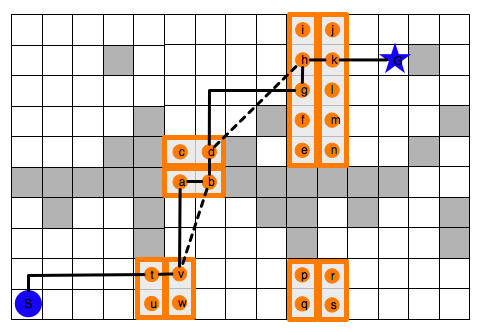
\includegraphics[scale=0.35, trim = 20mm 9mm 20mm 0mm]{diagrams/refinementexample.png}
       \end{center}
       \label{ia-fig:refinement}
	\vspace{-6pt}
\end{figure}

\subsection{Better heuristics}
We can use intervals to compute better heuristics to guide a low-level search.
$h(n) = g(nextentrance, goal) + manhattan(n, nextentrance)$

